% This is "aamas2009example.tex" Sept 2009
% This file should be compiled with "aamas2009.cls" or "aamas2009-extendedabs.cls" Sept 2007
%
% This example file demonstrates the use of the 'aamas2009.cls', or 'aamas2009-extendedabs.cls', resp.
% LaTeX2e document class file. It is for those submitting
% articles to AAMAS 2009 Proceedings. This file is based on
% the sig-alternate.tex example file.
% The 'sig-alternate.cls' file of ACM will produce a similar-looking,
% albeit, 'tighter' paper resulting in, invariably, fewer pages.
% than the original style ACM style.
%
% ----------------------------------------------------------------------------------------------------------------
% This .tex file (and associated .cls ) produces:
%       1) The Permission Statement
%       2) The Conference (location) Info information
%       3) The Copyright Line with AAMAS data
%       4) NO page numbers
%
% as against the acm_proc_article-sp.cls file which
% DOES NOT produce 1) thru' 3) above.
%
% Using 'aamas2009.cls' or 'aamas2009-extendedabs.cls' you don't have control
% from within the source .tex file, over both the CopyrightYear
% (defaulted to 200X) and the IFAAMAS Copyright Data
% (defaulted to X-XXXXX-XX-X/XX/XX).
% These information will be overwritten by fixed AAMAS 2009 information
% in the style files - it is NOT as you are used with ACM style files.
%
% ---------------------------------------------------------------------------------------------------------------
% This .tex source is an example which *does* use
% the .bib file (from which the .bbl file % is produced).
% REMEMBER HOWEVER: After having produced the .bbl file,
% and prior to final submission, you *NEED* to 'insert'
% your .bbl file into your source .tex file so as to provide
% ONE 'self-contained' source file.
%
% ================= IF YOU HAVE QUESTIONS =======================
% Questions regarding this AAMAS 2009 style, will be answered by
% the publication chair of AAMAS 2009 (publications@aamas2009.org)
% not by the ACM people that originally created the files.
% ===============================================================
%

% Use this for extended abstract submissions
%\documentclass{aamas2009-extendedabs}

% This is the document class for full paper submission
\documentclass{aamas2009}
%\documentclass[letterpaper]{aamas2009}

% if you are using PDF LaTex and you cannot find a way for producing
% letter, the following explicit settings may help
% \pdfpagewidth=8.5truein
% \pdfpageheight=11truein

\newenvironment{mylisting}
{\begin{list}{}{\setlength{\leftmargin}{1em}}\item\small\bfseries}
{\end{list}}

\begin{document}

% in the original styles from ACM, you would have needed to
% add meta-info here. This is not necessary for AAMAS 2009 as
% the complete copyright information is generated by the cls-files.

% For appropriate information about authors and title written in the
% copyright information, you must use these commands:

\AuthorsForCitationInfo{Simon Coakley}

\TitleForCitationInfo{Parallel agent communication and processing}


\title{Parallel agent communication and processing}

% \subtitle{(Extended Abstract)}
% Do NOT use any \subtitle command for EXTENDED ABSTRACT paper submissions.
% it will be overwritten by the text "(Extended Abstract)".

% AUTHORS

%\author{Tracking Number: 9999}
% For initial submission, do not give author names, but the
% tracking number, instead, as the review process is blind.

% You need the command \numberofauthors to handle the 'placement
% and alignment' of the authors beneath the title.
%
% For aesthetic reasons, we recommend 'three authors at a time'
% i.e. three 'name/affiliation blocks' be placed beneath the title.
%
% NOTE: You are NOT restricted in how many 'rows' of
% "name/affiliations" may appear. We just ask that you restrict
% the number of 'columns' to three.
%
% Because of the available 'opening page real-estate'
% we ask you to refrain from putting more than six authors
% (two rows with three columns) beneath the article title.
% More than six makes the first-page appear very cluttered indeed.
%
% Use the \alignauthor commands to handle the names
% and affiliations for an 'aesthetic maximum' of six authors.
% Add names, affiliations, addresses for
% the seventh etc. author(s) as the argument for the
% \additionalauthors command.
% These 'additional authors' will be output/set for you
% without further effort on your part as the last section in
% the body of your article BEFORE References or any Appendices.

\numberofauthors{1} %  in this sample file, there are a *total*
% of EIGHT authors. SIX appear on the 'first-page' (for formatting
% reasons) and the remaining two appear in the \additionalauthors section.
%
\author{
% You can go ahead and credit any number of authors here,
% e.g. one 'row of three' or two rows (consisting of one row of three
% and a second row of one, two or three).
%
% The command \alignauthor (no curly braces needed) should
% precede each author name, affiliation/snail-mail address and
% e-mail address. Additionally, tag each line of
% affiliation/address with \affaddr, and tag the
% e-mail address with \email.
%
% 1st. author
\alignauthor
Simon Coakley\\
       \affaddr{University of Sheffield}\\
       \affaddr{Kroto}\\
       \affaddr{Sheffield, UK}\\
       \email{s.coakley@shef.ac.uk}
}

%% There's nothing stopping you putting the seventh, eighth, etc.
%% author on the opening page (as the 'third row') but we ask,
%% for aesthetic reasons that you place these 'additional authors'
%% in the \additional authors block, viz.
%\additionalauthors{Additional authors: John Smith (The Th{\o}rv{\"a}ld Group,
%email: {\texttt{jsmith@affiliation.org}}) and Julius P.~Kumquat
%(The Kumquat Consortium, email: {\texttt{jpkumquat@consortium.net}}).}
%\date{30 July 1999}
%% Just remember to make sure that the TOTAL number of authors
%% is the number that will appear on the first page PLUS the
%% number that will appear in the \additionalauthors section.

\maketitle
\begin{abstract}

Modern developments in fields such as biology and economics mean that we have to
tackle the issue of extremely large amounts of data throughput. This is achieved
by providing efficient data transfer mechanisms and filters that permit the
operation of simulation environments featuring many thousands and millions of
agents. Executing large agent-based models requires large amounts of processing
power and memory which are not readily available on single computers. This paper
presents a formal specification of agents in an agent-based model such that the
description aids parallel execution.

% Submit to special area: Description Level: Methodologies/ Languages
% 
% Title:
% 
% Organising parallel processing of agents.
% 
% Defining agents for parallel execution and testing.
% 
% Managing massively multi agent systems to run on high performance computers eg
% blue gene

% This paper describes on going research as part of the E.U. funded EURACE project,
% to built a large scale agent-based model of the European economy able to run
% efficiently on high performance computers. New processing and communication
% strategies for parallel execution are described that utilise the many
% communication networks present in economic models.
% 
% Building on the FLAME which is based upon extended finite state machines
% (X-machines) where transitions between states are function that act on the
% memory of the machine and accept inputs and produce outputs.
% To keep synchronisation in parallel states can only be entered once.
% The level of model description of the transition functions is the sets of their
% input and output (obviously their current and next states) The lower level
% description of the functions is currently written in C.
% Currently being developed as part of the EURACE project. (web address?)
% Agent output is available to every other agent. Agent input can be restricted
% by the use of filters.
% Communication is 'broadcast', no point-to-point only communication (as don't
% know on which node an agent is (could keep records?))
% can use agent-to-agent communication by filtering input on identification
% numbers.
% 
% examples from economic models from EURACE:
% firms talking to households in same region
% ..
% 
% first used with biological modelling (cite Phil paper)
% where broadcast communication was mostly used..
% 
% The ordering of agent execution is dependent on the order of functions with each
% agent and also on the inputs and outputs between agents.
% 
% This can be calculated by working out the dependencies functions have on each
% other
% 1. state defined order with agents
% 2. communication between functions on specific message types
% , then for each processing step remove the functions that don't have any
% dependencies and add them to the current processing step. Repeat.
% 
% The order of function execution is calculated.
% 
% Execution in parallel requires communication be synchronised between processing
% parallel processing nodes.
% This is achieved using STFCs message passing library.
% Where calls are given to start a synchronisation and complete them..

\end{abstract}

% A category with the (minimum) three required fields
%\category{H.4}{Information Systems Applications}{Miscellaneous}
%A category including the fourth, optional field follows...
%\category{D.2.8}{Software Engineering}{Metrics}[complexity measures,
% performance measures]

%\terms{Delphi theory}

\keywords{parallel, synchronisation, process ordering}

\section{Introduction}

%Why research is novel and new and helps.

Modern developments in fields such as biology and economics mean that we have to
tackle the issue of extremely large amounts of data throughput. This is
achieved by providing efficient data transfer mechanisms and filters that permit the
operation of simulation environments featuring many thousands and millions of
agents. The diversity of potential applications in biology, including cellular
interactions \cite{3,125} and cell signalling pathways \cite{143}, and economics,
including modelling the European economy \cite{eurace01}, is large and therefore
a common formal development architecture is essential. This would provide a
platform for formally defined and analysable models which is essential for
satisfactory verification and validation. This is especially important for future
applications where models may play a part in drug development, economic policy
etc.

Executing large agent-based models requires large amounts of processing power
and memory which are not readily available on single computers. The use of high
performance computers with connected nodes of processors and memory requires
models to be executed in parallel, which fits the computational model of
autonomous agents acting within a network. To run models in
parallel they need to be formally defined and within parameters that allow
efficient execution techniques.

%To execute an agent-based model efficiently in parallel and to be able to
%verify and validate it, a formal description of the model is required.


This paper presents a formal specification of agents in an agent-based model
such that the description aids parallel execution. Techniques for efficient
parallel agent communication and processing are also presented. The key
contributions are:

\begin{enumerate}
  \item A model for formally specifying agents.
  \item A strategy for efficient parallel agent communication.
  \item A strategy for efficient parallel agent process ordering.
\end{enumerate}

% The techniques described in this paper are based upon a parallel agent platform. 
% The requirement for the agent platform to be parallel is two-fold, processing
% time and memory requirements. Both being limitations for simulation execution
% on single machines for large models. The machines that the platform is aimed
% at are high performance computers with hundreds and possibly thousands of
% processors, including the IBM Bluegene architecture.

% The need to go parallel is required not just by processing time issues but
% memory issues aswell where a single machine doesn't have enough memory to hold
% the entire simulation in one go.

\section{Background}

This research is funded by the European Union via the EURACE project which aims
to build a large scale agent-based model of the European economy to aid
economic policy design. The project requires the development of software techniques and
a software platform for large-scale agent-based economic simulations.

The issues involved include the definition of formal languages for modelling
and for optimising simulation execution.
Different formal description of agents have been proposed but none with the
onward ability to handle efficient parallel execution. UML has be proposed as a
formal language for the intermediate stage towards the implementation of a model
from its comceptualisation. But this does not provide implementation details and
parallel execution techniques. Other formal specification languages
\cite{object-z_statecharts, slabs} also do not give details on parallel
implementation.

Previous work on techniques and
a software platform for large-scale agent-based modelling of biological systems
has been developed at Sheffield University \cite{179, 256, 221}. Using abstract state
machines (X-machines) as the formal definition language for agents, which are
marked-up in XML, a parser was used, along with template files, to produce simulation code.
The parser has the ability to produce simulation code that works in parallel,
using the MPI library. The communication strategy used was limited to Cartesian
space as this was the common topology used in biological models. Each
processing node on a parallel computer has associated message boards where
agents post messages. When all agents have posted a message of a certain type,
the message boards are sychronisated in such a way that only messages required
by agents on a processing node are sent to the cooresponding node message
boards.
% why econmic models need more

Communication in economic models though are not resticted to
a topology-based network but economic activity involving many
heterogeneous agents with interconnected markets.


\subsection{X-Machines as Agent Specification}

For an efficient parallel agent-based model, the operating limits of agents
must be defined.
The following are the parameters used to define agent-based models used in this
paper:

% (The main factor of parallel efficiently is the commuication
% between computational nodes, or agent communication.)

\begin{enumerate}
  \item Agents can only communicate via messages. No agent can directly access
  another agent as they might not be located on the same computational node.
  \item Agent communication needs to be synchronised between computational nodes
  so agents have access to all avaliable messages. The results of a simulation
  should not be affected by the number of
computational nodes, or the node communication network, the simulation is
executed on.
  \item Agent processes need to be synchronised between computational nodes so
  that communication can be synchronised.
\end{enumerate}

%Model descriptions are currently written in XML for easy parsing.

%\subsection{Agent Specification}

% For an agent-based model to be executable in parallel, agents can only
% communicate via messages (or medium that can be sent between nodes on a
% parallel computer) and not directly access other agents. If anything in the
% environment of the model can be dynamic this must also be represented by an
% agent with communication via messages. This is because the environment might be
% held an a different node from agents that need to interact with it. Finally
% communication must be synchronised at certain points so that all agents can
% receive all available messages. This is so that the results of simulations are
% not affected by the number of nodes or hardware that the simulation is run on.

Each type of agent
is formally described as an abstract state machine, where transitions
between states are functions that can accept input and produce output and
update the memory of the machine. This type of machine is known as the
X-machine computational model Elienberg (1974) and has been proposed for
software specification and testing \cite{HOLCOMBE:1986} and verifying swarm
satellite systems at NASA \cite{162}.

% The interaction of agents is exclusively by messages. Agent function input and
% output is defined as being of message types, each having their own defined
% memory. Therefore models are defined by the agents types and message types.

Agent memory is defined by variables with C standard data types or any abstract
data types predefined by the modeller. Messages types which must also be
specified are defined in the same way.

Agent functions are defined by their transitions between states, any guard
conditions, the set of possible input messages and output messages, and any
changes in the agent memory. This information can usually be defined in a state
transition table where where $M_{pre}$ is the pre-condition of the memory (the
guard condition) and $M_{post}$ is the post-condition of the memory (any memory
updates), see Table \ref{tab:funcparameters}.

\begin{table}[hbp]
\centering
\begin{tabular}{|l|l|l||l||l|l|l|}
\hline
Current&Input&$M$&Func-&$M$&Output&Next\\
State&&$pre$&tion&$post$&&State\\
\hline
\end{tabular}
\caption{Function parameters} \label{tab:funcparameters}
\end{table}

The software platform currently reads models marked-up in XML and functions are
currently written as below where $M_{pre}$ is defined as \textit{condition} and
$M_{post}$ is written as C source code within a function with the same name as
the function name. This source code function reads agent memory, loops though
the input messages, sends output messages, and updates agent memory.

\begin{mylisting}
\begin{verbatim}
<function>
 <name>Function_name</name>
 <description>Description of the function</description>
 <currentState>current_state</currentState>
 <nextState>next_state</nextState>
 <condition>condition</condition>
 <inputs>inputs</inputs>
 <outputs>outputs</outputs>
</function>
\end{verbatim}
\end{mylisting}

An example model specification is given in Table \ref{tab:simpleexample} with
the cooresponding state diagram in Figure \ref{tab:simpleexample} showing a
single agent type that sends a message type between two functions. In a
simulation multiple agents of this type would send messages and receive each
others messages (as well as their own).

\begin{table}[hbp]
\centering
\begin{tabular}{|l|l|l||l||l|l|l|}
\hline
Current&Input&$M$&Func-&$M$&Output&Next\\
State&&$pre$&tion&$post$&&State\\
\hline
\hline
Start&&&Func-&&M&State\\
&&&tion 1&&&1\\
\hline
State&M&&Func-&&&End\\
1&&&tion 2&&&\\
\hline
\end{tabular}
\caption{Example model with one agent type sending and receiving a message
between two functions}
\label{tab:simpleexample}
\end{table}

\begin{figure}[hbp]
\centering
%\includegraphics[width=\columnwidth]{stategraph.ps}
\includegraphics[width=1.5in]{example_1.ps}
\caption{Example model with one agent type sending and receiving a message
between two functions}
\label{fig:simpleexample}
\end{figure}

The current EURACE economic model has 9 agent types with 159 functions using 55
message types to communicate. The complexity of the model can be seen in the
model state diagram, see Figure \ref{fig:eurace}.

\subsection{The Challenge of Concurrent X-Machine Communication}

% Problem
Handling communication efficiently between agents is a hard problem especially
in parallel. The emergent behaviour that make agent-based models appealing are
usually the result of local interactions which involve restricting
communication in a model, therefore making communication more managable.
% Context
Common solutions involve the use of grid-based spacial topologies, where
certain grid points can only communicate to a subset of other grid points that
are spacially near. Agents are then associated with grid points.
This solution only allows one communication network strategy and one
communication restriction, which are spacially based.
Spacial topology is less relivant for economic models looking to model economies
because the relationship between agents are based upon their economic activities
and not the spacial distance they are away from each other. For example: firms
employ households; households buy goods from firms; firms and households pay
taxes to the goverment; etc. Although the inclusion of ecomomic regions can
provide a spacial aspect if used. This implies that there are many
communication networks in economic models, specifically markets: labour; goods;
credit; financial; and economic regions.

\section{Managing Concurrent\\Agent Communications}

A new communication strategy was needed that allows generic communication
networks with generic communication restrictions.
A new parallel communication library was developed based upon filters and the
starting and completion of message synchronisation.

\begin{figure}[hbp]
\centering
%\includegraphics[width=\columnwidth]{stategraph.ps}
\includegraphics[width=2in]{layer_model.eps}
\caption{Layered architecture}
\end{figure}

The current design of the framework consists of a model specification
describing abstract state machines for each agent in a model along with
the implementation of agent functions in source code. The framework parser reads
the model specification, calculates order of operations, and produces simulation
source code which is compiled with the agent function source code and linked
with the communication library.

\subsection{Type-Based Message Filtering}

The model specification already defines a communication restriction: message
types that can be sent between certain agent types. For example firms sending
\textit{job vacancy} messages to households.
This level of information can be used to inform the partitioning strategy of
agents where agents types that often communicate are placed on the same
processing node, therefore limiting node to node communication.

But there is always going to be communication between processing nodes and the
more this can be restricted the less data that needs to be exchanged and the
more efficient the execution of a model will be.

% More restrictions the
% better to try and limit the amount of communication exchanged between
% processing nodes.



%The strategy proposed in this paper is the use of broadcast communication and
%the use of filters.

% This is a good strategy for biological models which are spacially based.
% With respect to economic models, agent communication is less spacially based,
% with more emphesis on markets involving different types of agents, for example:
% labour with firms households; goods with firms malls and households; credit
% with banks; firms and households, etc.
% % Solution
% The communication strategy needs to be more generic with multiple communication
% networks, for example firms and households interact within many market types.
% 
% One of the added problems with parallel execution is that it can be
% preventative to use direct communication as this would require tracking every
% agent in a simulation (and giving its location on a computing node).

% Between outputs of a message type and its inputs there needs to be a
% synchronisation of messages between computing nodes.
% 
% Not all messages are required by all agents, dependent on some filter, so the
% sending of all messages to all computing nodes can be restricted.
% 
% The more filters the better not just topology based.
% 
%  Filters can be about more than topology so
% the more filters that can be defined the less messages that need to be
% synchronised across computational nodes. For example:

The communication restriction strategy uses filters for function input, not just
for local interactions, but generic comparisions between agent memory
and message memory.

Filters are built up from conditions on variables from messages where the
operator can be one of:

\begin{itemize}
  \item EQ -- equals
  \item NEQ -- not equal
  \item LT -- less than
  \item GT -- greather than
  \item LEQ -- less than or equal
  \item GEQ -- greather than or equal
\end{itemize}

Conditions can also be build up using \textit{and} and \textit{or} logical
operators.

For example:

\begin{itemize}
  \item When households read job vacancy messages from firms they only want to
  read vacancies that contain a wage level above a certain level:\\
$message\_wage\_level >= agent\_required\_wage\_level$
  \item When firms read job application messages from
households they want applications related to their vacancies:\\
$message\_firm\_vacancy\_id == agent\_firm\_id$
\end{itemize}

The design of the communication library provides the ability to register
filters with associated parameters, and methods to start a synchronisation and
ask for a synchronisation completion before the messages are required to be
read.

A synchronisation without filters will invoke the communication library to send
all messages from the local message board to all other processing nodes.

By registering a filter before a synchronisation the communication library
requires processing nodes to send their filter parameters to other nodes who
use this information along with the filter to restrict outgoing data.

The parameters required for filters can be easily reduced for each processing
node. For example where the filter operation is:

\begin{itemize}
  \item EQ / NEQ - the list of unqiue values is required
  \item LT / LEQ - the maximum value is required
  \item GT / GEQ - the minimum value is required
\end{itemize}

For more complicated filters that require functions, for example
two-dimentional Cartesian space, the parameters required would be:

\begin{itemize}
  \item minumum and maximum x-axis values
  \item minimum and maximum y-axis values
\end{itemize}

These filters also guide parallel partitioning strategies. For example if many
filters filter using a region identification number then this suggests agents
should be partitioned according to the value of that particular variable in
their memory.

% Every function that accepts the input of a message type requires a
% synchronisation with the message board.
% These synchronisations can be batched together..

\subsection{Ensuring Consistent\\Distributed Execution}

The sychronisation of communication requires the sychronisation of processing
nodes and therefore the agents being processed.
Each agent is defined as an abstract state machine therefore the execution of 
state transitions of agents need to be ordered and kept the same on each
processing node.

% Each agent state is implemented as a list.
% Agents are moved between states after they have run certain functions.
% When all agents have reached an end state, the iteration is finished.
% The order that agent are moved and functions executed is the process order.

% Each agent type has its order defined by the transition functions between
% states. There can only be one start state, many end states, and to keep agents
% synchronised in parallel states can only be entered once.

A dependency graph of agent functions can be created which guides the execution
order. There are two types of dependencies:

\begin{itemize}
  \item Internal - a function exiting state \textit{s} depends on all functions
  entering \textit{s}
  \item Communication - a function accepting input of message type \textit{m}
  depends on all messages outputting the message type \textit{m}.
\end{itemize}

By removing functions with no dependencies from the dependency graph and placing
them in the first execution layer, then removing the remaining functions and
placing them in the next execution layer, and so on until there are no
functions left in the dependency graph, one can create an execution order that
will execute a model correctly.

For example the model in Figure \ref{fig:stategraph_1} would create the
dependency diagram in Figure \ref{fig:dgraph_1} which shows the execution
layers of functions. The black edges/arrows are internal dependencies and the
green edges/arrows show the communication dependencies via the parallelogram
showing the message type. The dependency graph also shows that a commuication
sychronisation must take place between execution layers 2 and 3.

The current EURACE model, see Figure \ref{fig:eurace}, has 75 execution layers.

\begin{figure}[hbp]
\centering
\includegraphics[width=2in]{stategraph_1.ps}
\caption{Model state diagram}
\label{fig:stategraph_1}
\end{figure}

\begin{figure}[hbp]
\centering
\includegraphics[width=2in]{dgraph_1.ps}
\caption{Model dependency diagram}
\label{fig:dgraph_1}
\end{figure}

The execution order can be made more efficient by providing the maximum possibe
time for communication sychronisations by moving agents that output messages to
the start and moving agents that receive input messages to the end. In relation
to the functions in execution layer 2 it would be better to execute function FB2
on agents before executing function FA1. By executing agent functions during
synchronisations it means processing nodes are not idling waiting for
commonication to complete.
And by processing functions during communication sychronisations no processing
time is wasted.

%If functions use one can try 




% Process ordering is also governed by the communication of
% agent, their function inputs and outputs. Before any inputs can occur of a
% certain message type all outputs must occur before hand. Then the time between
% the last output and each input of a message type a message board
% synchronisation must occur. This is to synchronise messages between nodes in
% parallel.
% 
% Ordering processes to help efficiently:
% 
% Process other functions while doing communication syncs.
% Start syncs as soon as possible.
%   Have to start after last output.
%   If filters wait until smaller amount of agents in state before?
% Complete syncs as late as possible.

% \begin{figure}[hbp]
% \centering
% %\includegraphics[width=\columnwidth]{stategraph.ps}
% \includegraphics[width=2in]{stategraph.ps}
% \caption{An example state diagram}
% \end{figure}

\begin{figure}[hbp]
\centering
%\includegraphics[width=\columnwidth]{stategraph.ps}
\includegraphics[totalheight=0.96\textheight]{eurace_stategraph.ps}
\caption{EURACE state diagram}
\label{fig:eurace}
\end{figure}


%\end{document}





% First the agent description is described, which includes how agents need to
% operate to work in parallel: broadcast communication, no direct agent
% connections, no entering same state twice to keep nodes synchronised.
% 
% Second describe how agent execution order is calculated.
% 
% 
% 
% Use of this framework for testing see this paper using Daikon \cite{289}

\section{Discussion}

When executing large scale models on parallel computers a strategy is required
to keep the model syncronised between processing nodes and restrict the amount
of node to node communication as much as possible.
The use of formally defined agents provides a way to pre-define agent
function processing, keeping processing nodes synchronised, and calculating
efficient times to sychronise communication between processing nodes.
The use of input filters for agent functions provides a generic way to restrict
agent communication while implicitly creating communication networks that can
guide parallel partitioning strategies.


% Related work / conclusions and future work

% No spacial topologies explicit, but implicit via the use of input filters used by
% agents.

%ACKNOWLEDGMENTS are optional
\section{Acknowledgements}
We would like to thank our EURACE colleagues for guiding the requirements for a
large scale economic model and
we gratefully acknowledge the research funding by the European Commission as
part of the FP6-STREP project EURACE (under contract no. 035086).

%
% The following two commands are all you need in the
% initial runs of your .tex file to
% produce the bibliography for the citations in your paper.
\bibliographystyle{abbrv}
\bibliography{coakley_aamas2009}  % sigproc.bib is the name of the Bibliography in this case
% You must have a proper ".bib" file
%  and remember to run:
% latex bibtex latex latex
% to resolve all references
%
% ACM needs 'a single self-contained file'!
%
%APPENDICES are optional
%\balancecolumns
% \appendix
% %Appendix A
% \section{Headings in Appendices}
% The rules about hierarchical headings discussed above for
% the body of the article are different in the appendices.
% In the \textbf{appendix} environment, the command
% \textbf{section} is used to
% indicate the start of each Appendix, with alphabetic order
% designation (i.e. the first is A, the second B, etc.) and
% a title (if you include one).  So, if you need
% hierarchical structure
% \textit{within} an Appendix, start with \textbf{subsection} as the
% highest level. Here is an outline of the body of this
% document in Appendix-appropriate form:
% \subsection{Introduction}
% \subsection{The Body of the Paper}
% \subsubsection{Type Changes and  Special Characters}
% \subsubsection{Math Equations}
% \paragraph{Inline (In-text) Equations}
% \paragraph{Display Equations}
% \subsubsection{Citations}
% \subsubsection{Tables}
% \subsubsection{Figures}
% \subsubsection{Theorem-like Constructs}
% \subsubsection*{A Caveat for the \TeX\ Expert}
% \subsection{Conclusions}
% \subsection{Acknowledgements}
% \subsection{Additional Authors}
% This section is inserted by \LaTeX; you do not insert it.
% You just add the names and information in the
% \texttt{{\char'134}additionalauthors} command at the start
% of the document.
% \subsection{References}
% Generated by bibtex from your ~.bib file.  Run latex,
% then bibtex, then latex twice (to resolve references)
% to create the ~.bbl file.  Insert that ~.bbl file into
% the .tex source file and comment out
% the command \texttt{{\char'134}thebibliography}.
% % This next section command marks the start of
% % Appendix B, and does not continue the present hierarchy
% \section{More Help for the Hardy}
% The aamas2009.cls and aamas2009-extendedabs files are based on the
% sig-alternate.cls file that is itself chock-full of succinct and
% helpful comments.  If you consider yourself a moderately experienced
% to expert user of \LaTeX, you may find reading it useful but please
% remember not to change it.
\balancecolumns % GM June 2007
% That's all folks!
\end{document}
